% Created 2024-03-22 Fri 04:54
% Intended LaTeX compiler: pdflatex
\documentclass[11pt]{article}
\usepackage[utf8]{inputenc}
\usepackage[T1]{fontenc}
\usepackage{graphicx}
\usepackage{longtable}
\usepackage{wrapfig}
\usepackage{rotating}
\usepackage[normalem]{ulem}
\usepackage{amsmath}
\usepackage{amssymb}
\usepackage{capt-of}
\usepackage{hyperref}
\usepackage[backend=bibtex, style = authoryear-comp]{biblatex} % For IEEE numbered headings, use [backend=bibtex,block = ragged, style = numeric, sortcites]
\author{Guanghao Jiao}
\date{\textit{<2024-03-22 Fri>}}
\title{RIMANUS Meeting 20240322}
\hypersetup{
 pdfauthor={Guanghao Jiao},
 pdftitle={RIMANUS Meeting 20240322},
 pdfkeywords={},
 pdfsubject={},
 pdfcreator={Emacs 29.2 (Org mode 9.6.15)}, 
 pdflang={English}}
\begin{document}

\maketitle

\section{Scenario: Unprotected Loss of Flow (ULOF) in SFR (Almost impossible)}
\label{sec:org40b54c4}
\begin{itemize}
\item Complete failure of redundant shutdown systems
\item Failure forced circulation (e.g. Station Blackout)
\item Thermal mixing happens primarily due to natural convection
\end{itemize}

\section{What is the natural circulation/convection?}
\label{sec:orgf14a69d}
\begin{itemize}
\item Sodium: high thermal conductivity
\item Thermal stratification in sodium pool
\item Induced by temperature difference of coolant at the inlet and outlet of the core
\item Temperature difference --> Density difference --> Convection
\item Decay heat removed without electricity
\item One of the most important mechanisms of passive safety
\end{itemize}

\section{How fast is the natural convection?}
\label{sec:orgc34b094}
\begin{itemize}
\item Locally different
\item No more than 0.6m/s
\item Lack of study until 2022
\end{itemize}

\section{From natural circulation to \href{20240307154931-core_disruptive_accident_cda.org}{Core Disruptive Accident (CDA)}}
\label{sec:orgb3688b5}
\begin{itemize}
\item 15 hours from failure of forced circulation to total sodium boiling without natural circulation
\end{itemize}

\section{What is the process of CDA?}
\label{sec:org48fa77d}
\begin{itemize}
\item Initial Phase (IP)
\item Transition Phase (TP)
\item Post-Accident Material Relocation/Post-Accident Heat Removal (PAMR/PAHR) phase
\item \href{images/CDA.png}{Sketch of CDA}
\begin{center}
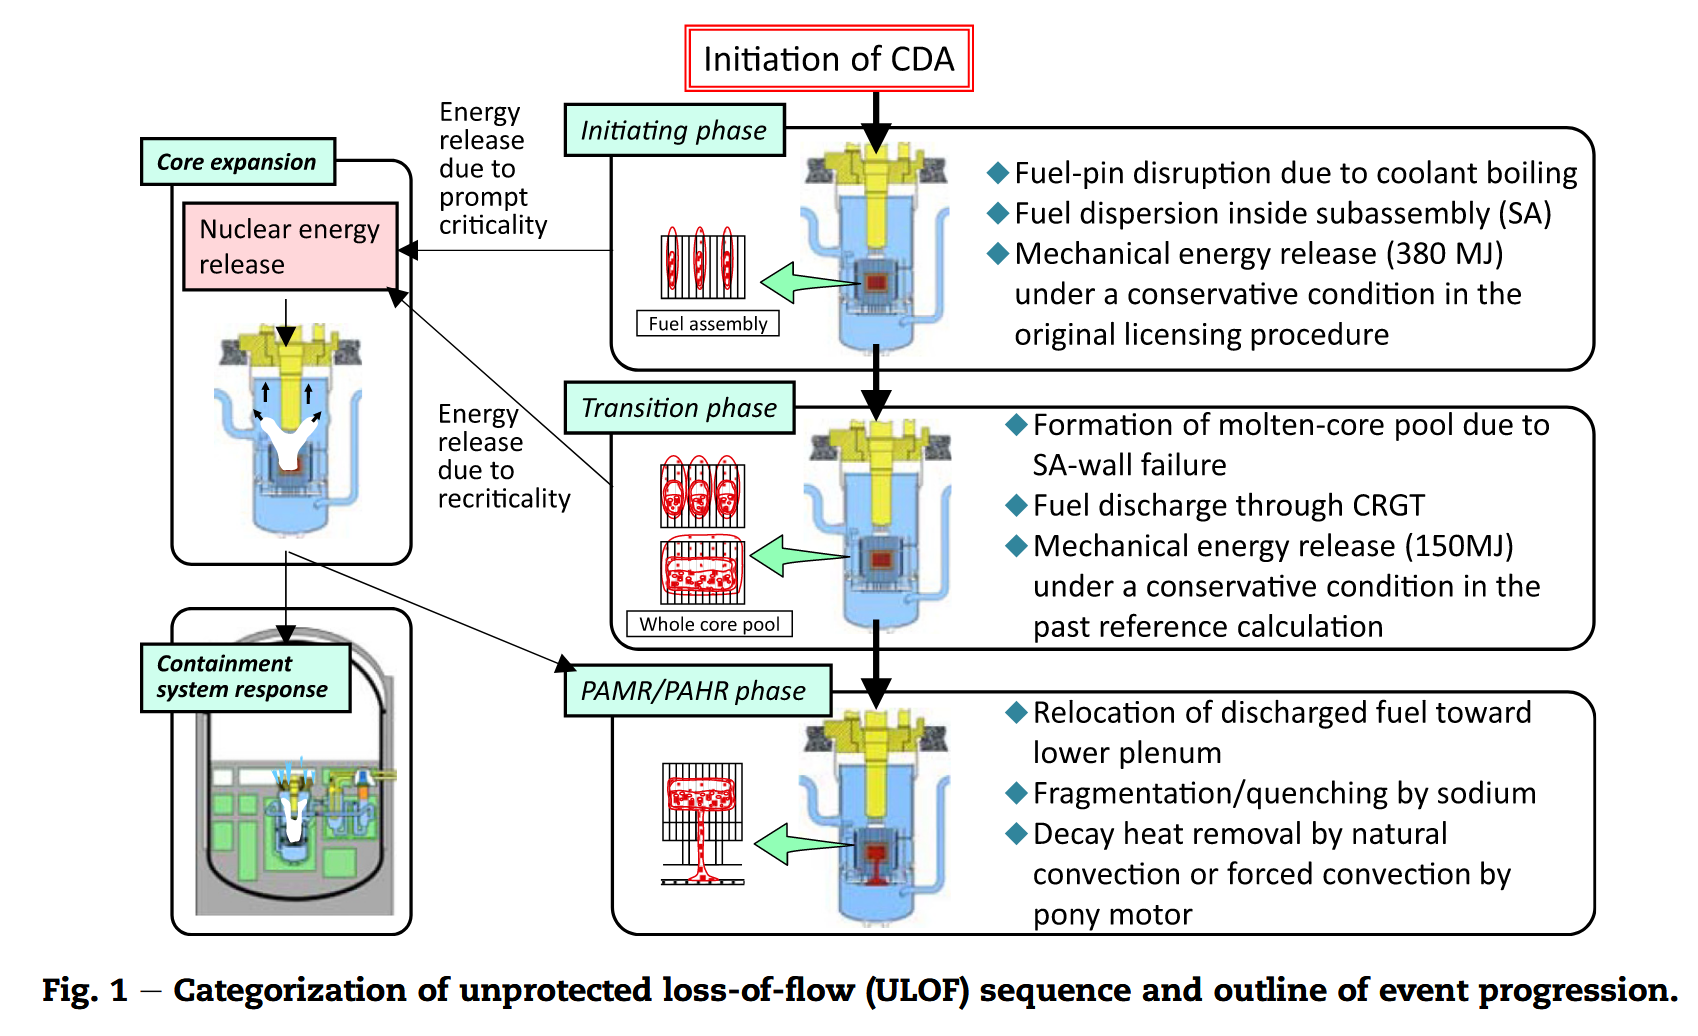
\includegraphics[width=.9\linewidth]{images/CDA.png}
\end{center}
\item \href{images/framework\_code.png}{Components of the meltdown}
\begin{center}
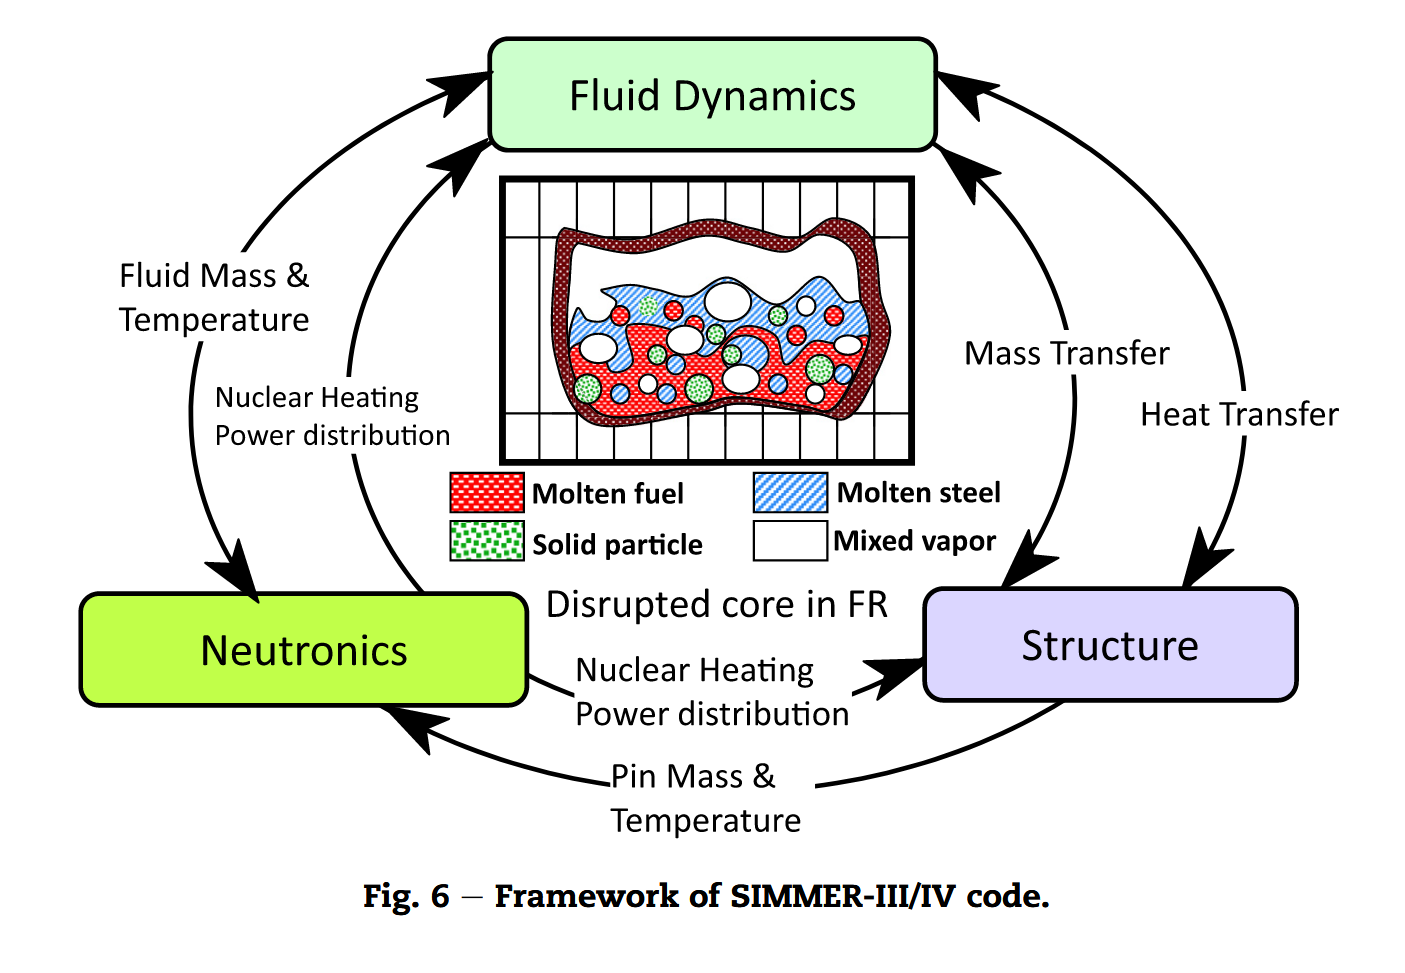
\includegraphics[width=.9\linewidth]{images/framework_code.png}
\end{center}
\item \href{images/transient.png}{Transient of reactivity and power in initiating phase}
\begin{center}
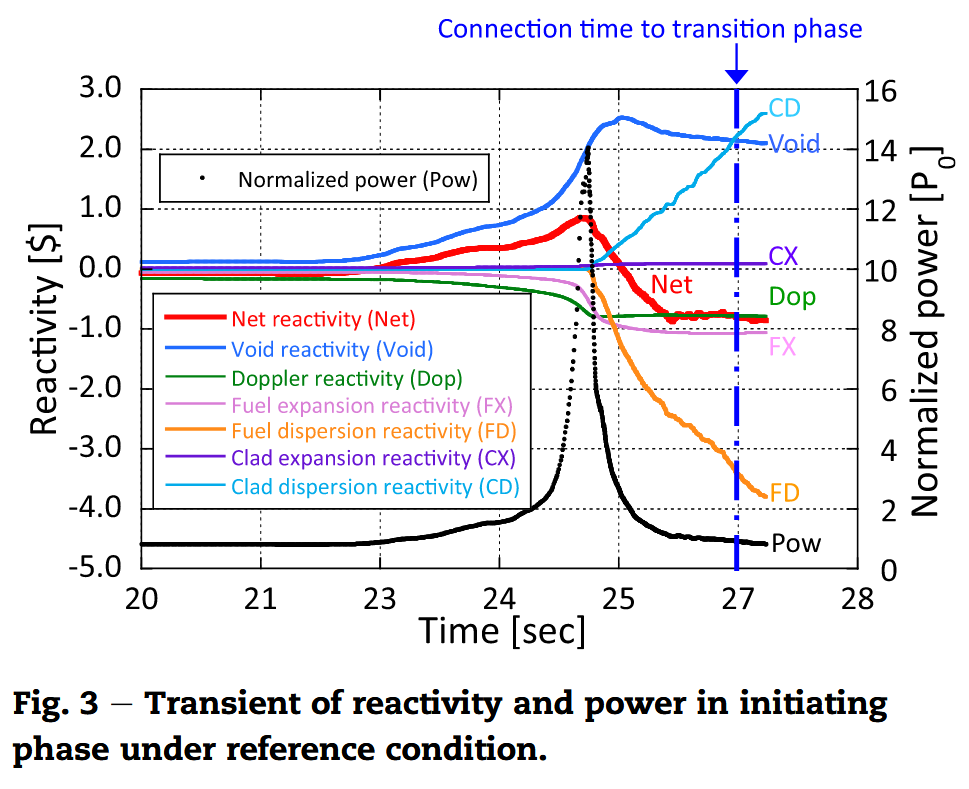
\includegraphics[width=.9\linewidth]{images/transient.png}
\end{center}
\item \href{images/components.png}{Components of the mixture}
\begin{center}
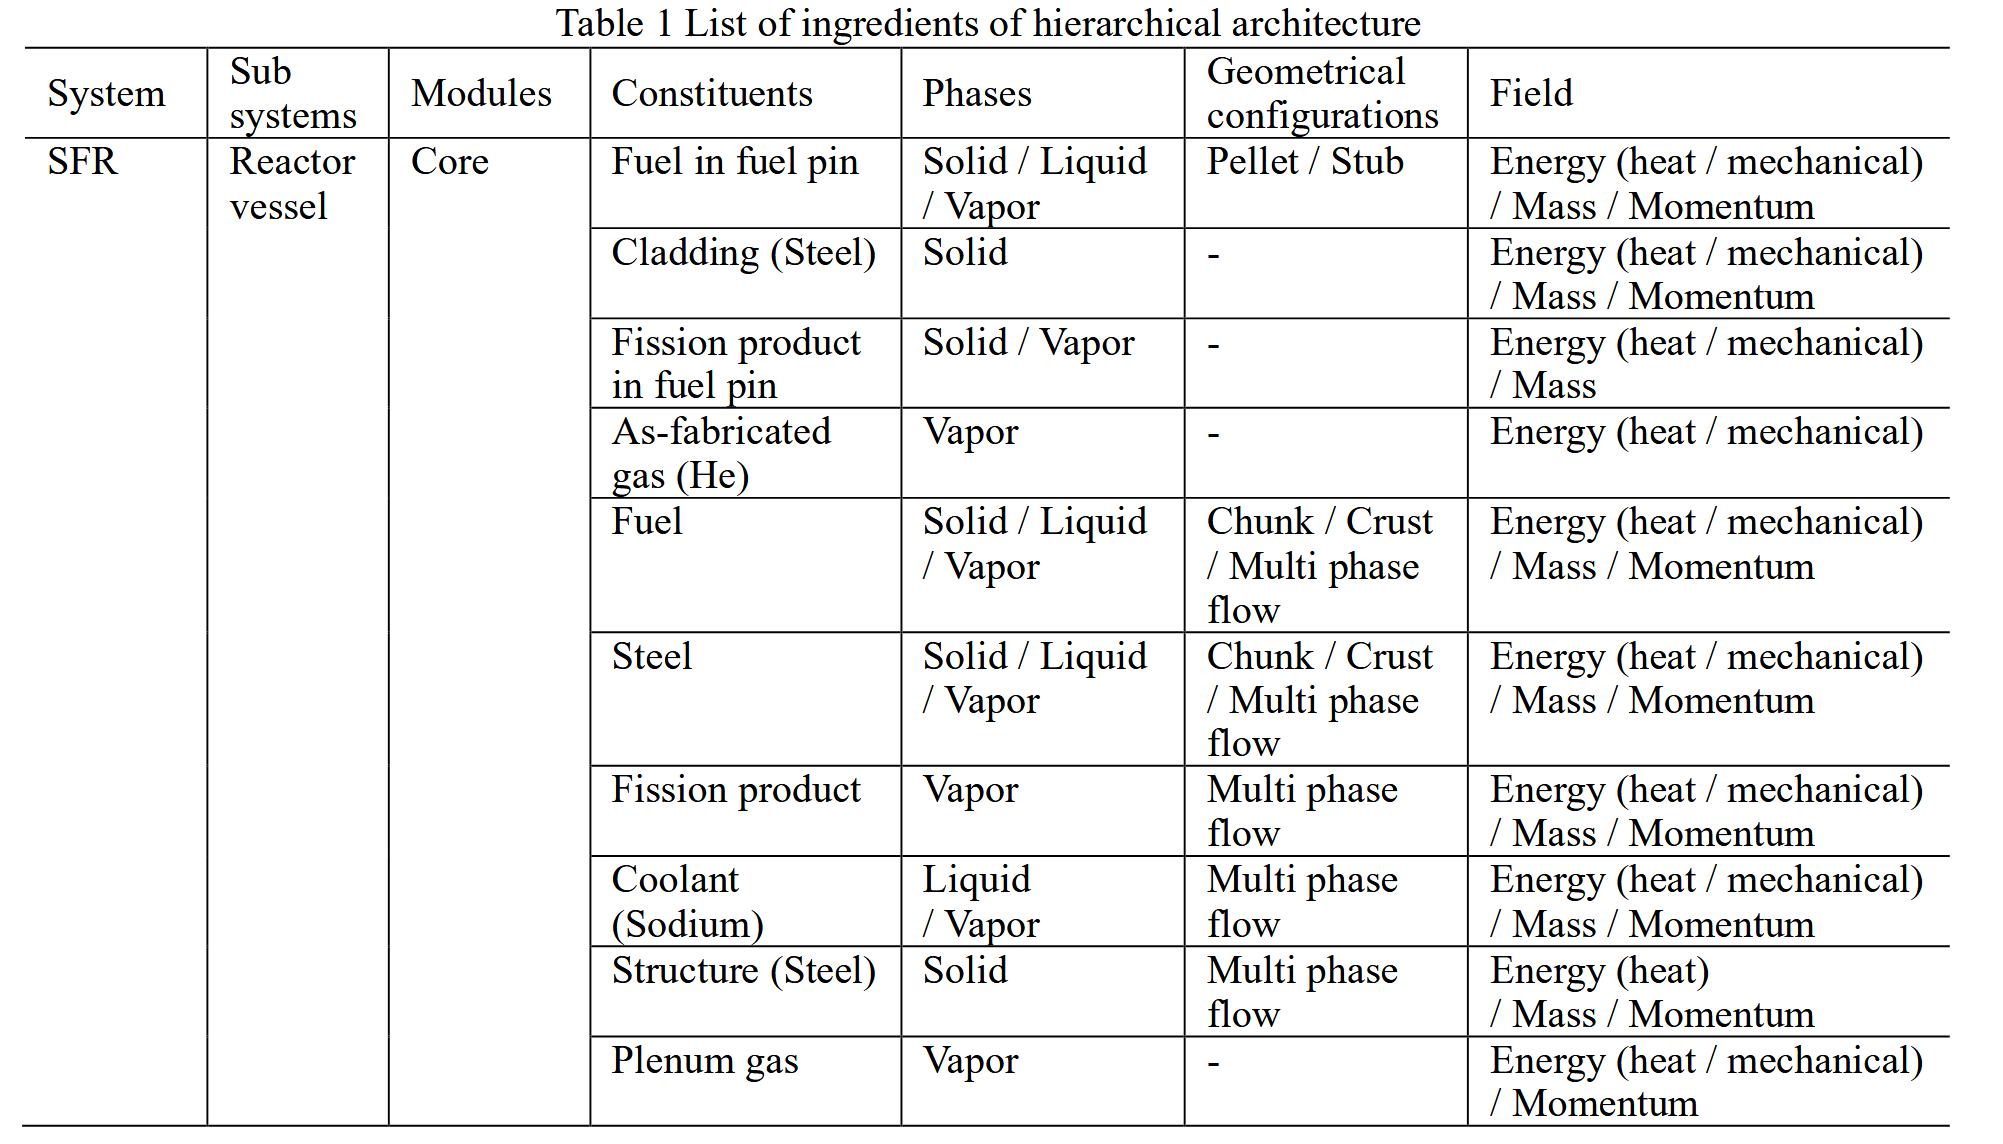
\includegraphics[width=.9\linewidth]{images/components.png}
\end{center}
\end{itemize}

\section{About viscosity}
\label{sec:org38e1160}
\begin{itemize}
\item \href{20240313140039-viscosity.org}{Viscosity} \(\uparrow\) Coalescence \(\downarrow\) (Important)
\end{itemize}

\section{Quotes}
\label{sec:org58a1fa5}
\begin{quote}
The reduction of the coolant flow causes (1) the fuel temperature rise and (2) the fuel thermal expansion, and the thermal expansion changes the fuel-cladding gap width. This change affects (3) the gap conductance and the thermal condition changes accordingly. The events progress while the thermal behavior and the mechanical behavior interact with each other. The coolant gradually boils and it causes the cladding temperature rise. In an assembly where the strength of the cladding is sufficiently degraded due to the temperature rise, (4) the fuel pellets temperature rises, the molten cavities develop, and (5) the fuel is disrupted when the fuel pellets cannot maintain their shape due to the strength degradation. Hence, the fuel disruption largely depends on the fuel pin thermal behavior and the fuel pin mechanical behavior. Furthermore, when the power excursion occurs due to the positive reactivity insertion which is caused by the coolant boiling, (6) the pressure applied by the fuel to the cladding, which is called the contact pressure, causes (7) the fuel pin failure in an assembly where the cladding keeps the strength due to sufficient cooling.
\end{quote}
\begin{quote}
Experiments show that the viscosity has a greater impact on the bubble coalescence. The greater the viscosity, the harder the bubbles are to coalesce.
\end{quote}
\section{Bibliography}
\label{sec:orga6b097a}
\printbibliography[heading=none]
\end{document}
